% 图 53.6 —— 由 `checks/emit_hand.py` 自动拼出（probe 精测 + prims2 图元分解）
%%
% ⚠ 这是**稿子不是成品**：跑 `checks/checkhand.py 53.6` 看指标 + 看叠合图。
%%
%% ⚠ 待核：
%   · 本图 probe 报出阴影族 1 个 —— **本脚本不生成阴影**（要照原书手写）；prims2 的 strokes 里可能含阴影线，核对时留意别画重
%   · 可疑字形 2 项（空心圈 ⊙ 常被认成字母 o）—— 见文件末
%%
\documentclass[12pt]{standalone}
\usepackage{fontspec}
\setsansfont{Arial}
\newfontfamily\mfallback{DejaVu Sans}
\usepackage{tikz}
\begin{document}
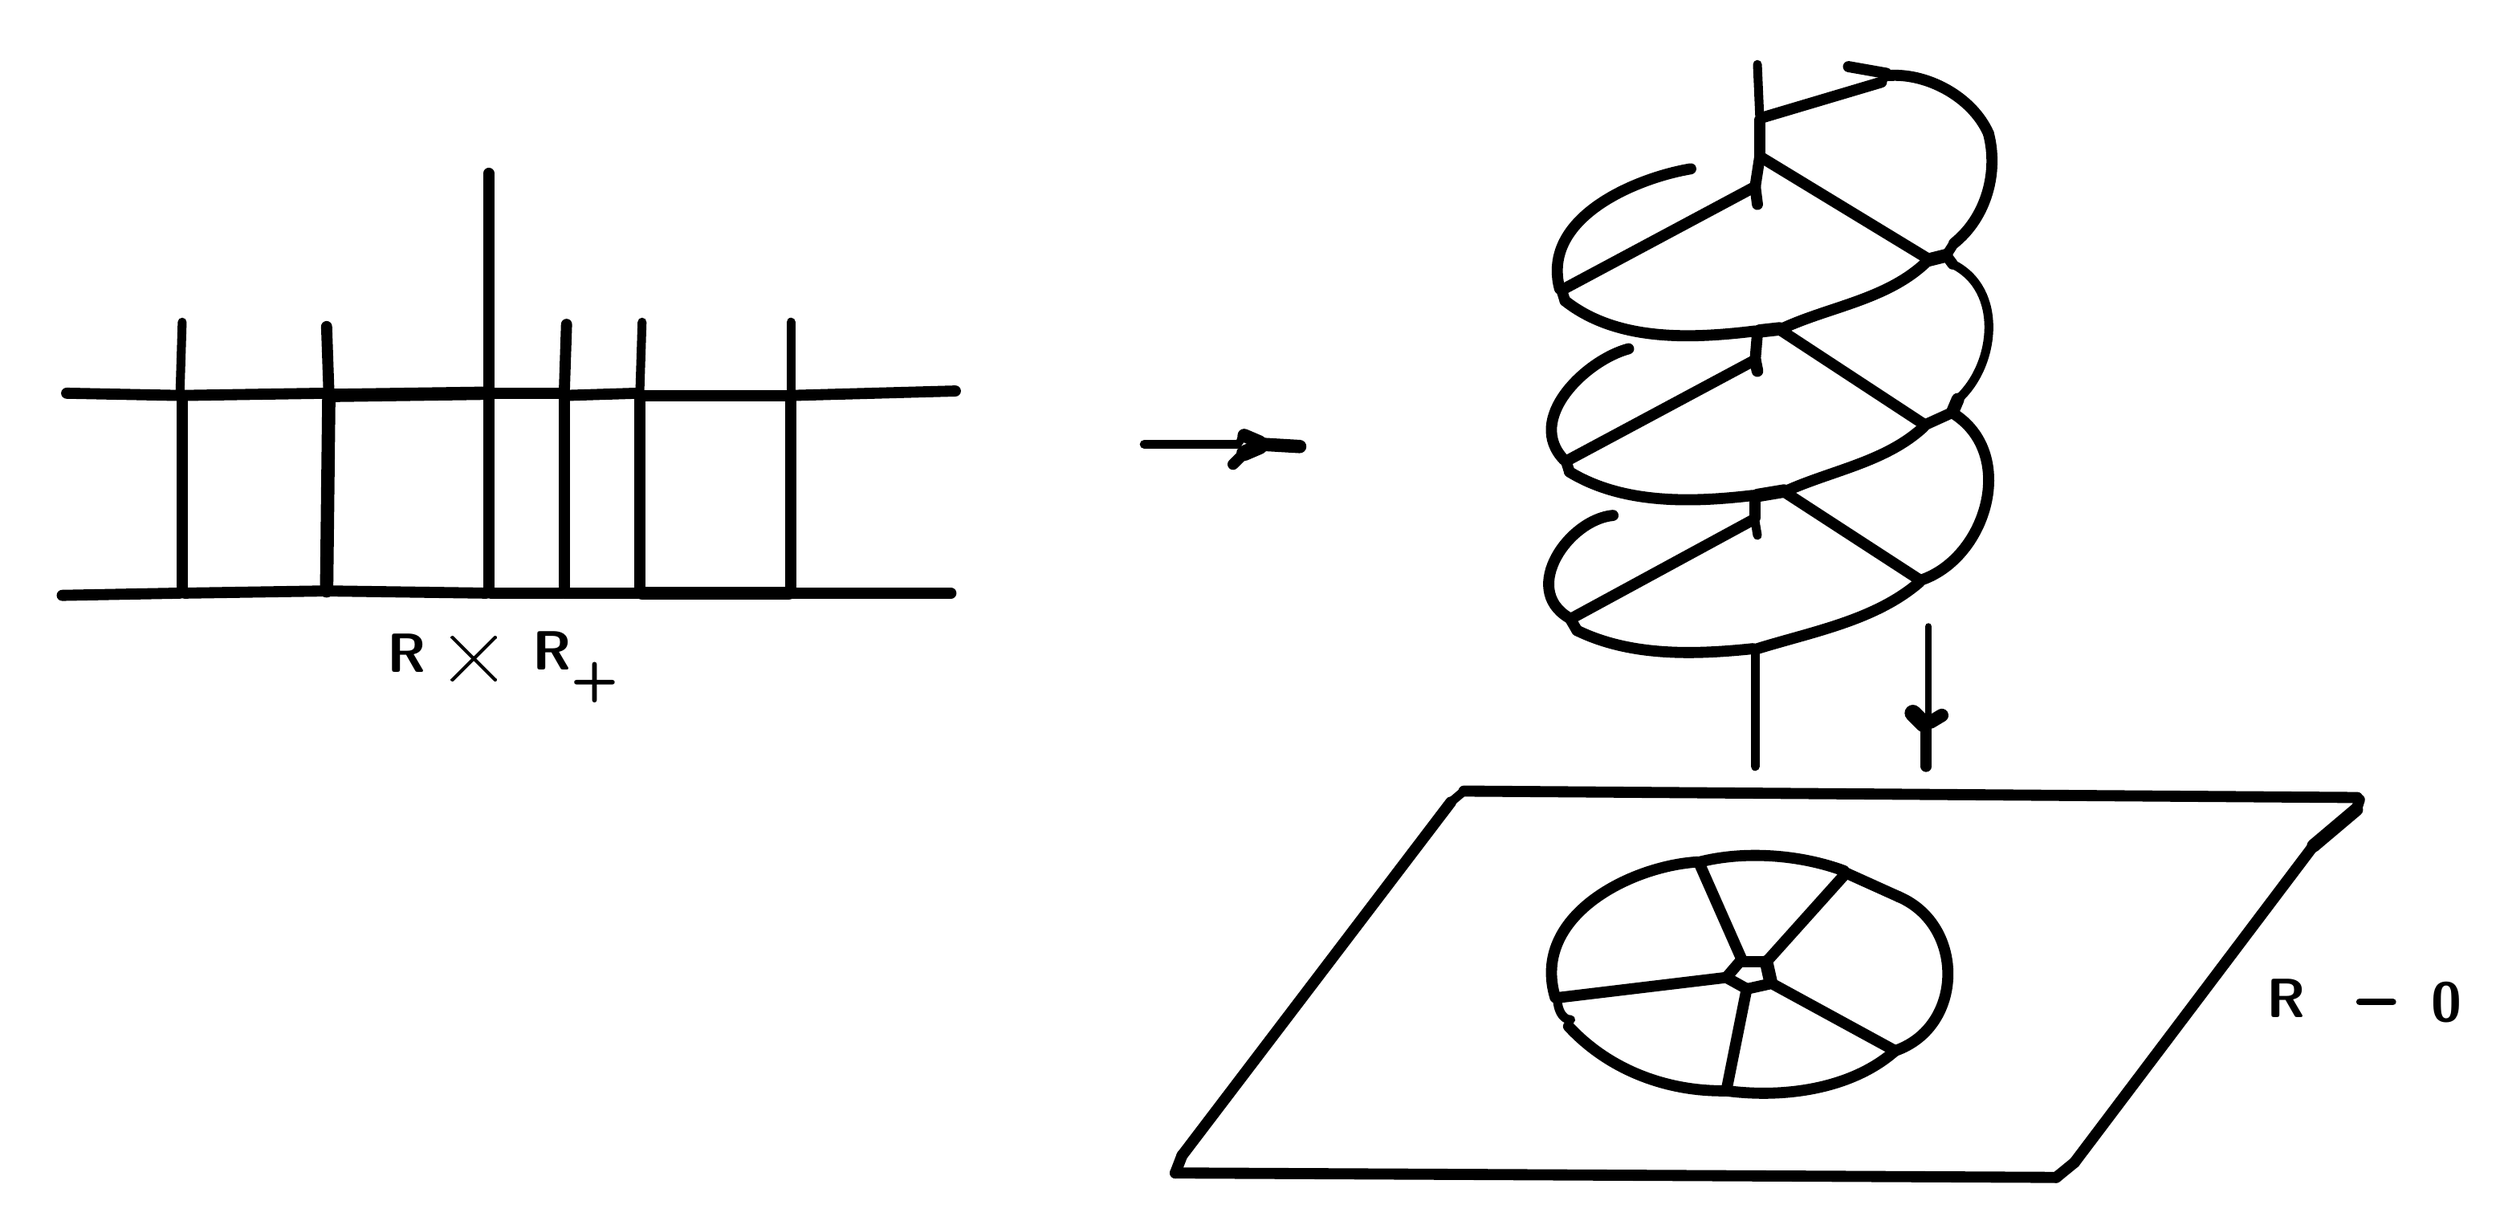
\begin{tikzpicture}[x=1pt, y=-1pt, line width=5.0pt, line cap=round, line join=round]

  %% ════ 直线段（prims2 的 strokes）════
  \draw[line width=5.0pt] (696.0,197.0) -- (780.0,152.0);
  \draw[line width=5.0pt] (210.0,68.0) -- (210.0,166.0);
  \draw[line width=4.9pt] (695.0,198.0) -- (696.4,202.4);
  \draw[line width=4.0pt] (547.0,190.0) -- (505.0,190.0);
  \draw[line width=5.0pt] (755.0,379.0) -- (774.0,422.0);
  \draw[line width=5.0pt] (822.0,20.0) -- (839.0,23.0);
  \draw[line width=3.4pt] (548.0,189.0) -- (549.0,186.0);
  \draw[line width=6.0pt] (782.0,139.0) -- (791.0,138.0);
  \draw[line width=6.0pt] (557.0,189.0) -- (550.0,186.0);
  \draw[line width=5.0pt] (72.0,169.0) -- (72.0,256.0);
  \draw[line width=5.0pt] (345.0,168.0) -- (279.0,168.0);
  \draw[line width=5.0pt] (20.0,167.0) -- (70.0,168.0);
  \draw[line width=5.0pt] (783.0,61.0) -- (857.0,106.0);
  \draw[line width=7.0pt] (557.0,191.0) -- (550.0,194.0);
  \draw[line width=7.5pt] (851.0,311.0) -- (856.0,316.0);
  \draw[line width=4.0pt] (780.0,283.0) -- (780.0,335.0);
  \draw[line width=5.0pt] (857.0,181.0) -- (868.0,176.0);
  \draw[line width=5.0pt] (73.0,168.0) -- (137.0,167.0);
  \draw[line width=5.0pt] (346.0,169.0) -- (346.0,256.0);
  \draw[line width=3.0pt] (1052.0,441.0) -- (1067.0,441.0);
  \draw[line width=5.0pt] (210.0,168.0) -- (210.0,256.0);
  \draw[line width=5.0pt] (820.0,384.0) -- (785.0,423.0);
  \draw[line width=5.0pt] (347.0,168.0) -- (420.0,166.0);
  \draw[line width=6.0pt] (138.0,169.0) -- (137.0,256.0);
  \draw[line width=5.0pt] (545.0,199.0) -- (549.0,195.0);
  \draw[line width=6.0pt] (139.0,168.0) -- (209.0,167.0);
  \draw[line width=3.0pt] (858.0,314.0) -- (858.0,272.0);
  \draw[line width=5.0pt] (857.0,317.0) -- (857.0,335.0);
  \draw[line width=5.0pt] (418.0,257.0) -- (347.0,257.0);
  \draw[line width=5.0pt] (244.0,257.0) -- (277.0,257.0);
  \draw[line width=5.0pt] (780.0,152.0) -- (781.0,140.0);
  \draw[line width=5.3pt] (780.0,152.0) -- (781.0,157.0);
  \draw[line width=6.0pt] (859.0,315.0) -- (864.0,312.0);
  \draw[line width=5.0pt] (843.0,463.0) -- (788.0,433.0);
  \draw[line width=5.0pt] (844.7,393.7) -- (821.0,383.0);
  \draw[line width=4.0pt] (781.0,19.0) -- (782.0,42.0);
  \draw[line width=5.0pt] (782.0,60.0) -- (782.0,44.0);
  \draw[line width=5.0pt] (785.0,423.0) -- (775.0,423.0);
  \draw[line width=6.0pt] (785.0,423.0) -- (787.0,432.0);
  \draw[line width=5.0pt] (777.0,435.0) -- (786.0,433.0);
  \draw[line width=4.0pt] (346.0,167.0) -- (346.0,135.0);
  \draw[line width=5.0pt] (137.0,256.0) -- (73.0,257.0);
  \draw[line width=5.0pt] (137.0,256.0) -- (209.0,257.0);
  \draw[line width=5.8pt] (869.0,175.0) -- (871.2,169.8);
  \draw[line width=4.9pt] (868.9,108.9) -- (866.0,105.0);
  \draw[line width=6.0pt] (558.0,190.0) -- (575.0,191.0);
  \draw[line width=5.0pt] (1051.0,349.0) -- (648.9,346.1);
  \draw[line width=4.0pt] (648.9,346.1) -- (643.0,351.1);
  \draw[line width=5.0pt] (643.0,351.1) -- (522.0,510.2);
  \draw[line width=5.0pt] (522.0,510.2) -- (519.0,518.0);
  \draw[line width=5.0pt] (211.0,167.0) -- (243.0,167.0);
  \draw[line width=5.0pt] (767.0,481.0) -- (776.0,436.0);
  \draw[line width=5.0pt] (780.0,214.0) -- (780.0,223.0);
  \draw[line width=3.8pt] (839.0,24.0) -- (836.8,27.0);
  \draw[line width=5.0pt] (836.8,27.0) -- (783.0,43.0);
  \draw[line width=4.0pt] (279.0,135.0) -- (278.0,166.0);
  \draw[line width=6.0pt] (793.0,211.0) -- (781.0,213.0);
  \draw[line width=4.9pt] (1052.0,350.0) -- (1050.6,354.4);
  \draw[line width=6.0pt] (1050.6,354.4) -- (1031.3,370.7);
  \draw[line width=5.0pt] (1031.3,370.7) -- (923.7,513.3);
  \draw[line width=5.0pt] (923.7,513.3) -- (915.5,520.0);
  \draw[line width=5.0pt] (915.5,520.0) -- (519.0,518.0);
  \draw[line width=5.0pt] (698.0,268.0) -- (779.0,224.0);
  \draw[line width=5.0pt] (697.0,269.0) -- (699.8,273.8);
  \draw[line width=5.0pt] (794.0,212.0) -- (854.0,251.0);
  \draw[line width=5.0pt] (773.0,423.0) -- (767.0,430.0);
  \draw[line width=5.0pt] (243.0,257.0) -- (211.0,257.0);
  \draw[line width=5.0pt] (244.0,166.0) -- (245.0,136.0);
  \draw[line width=5.0pt] (244.0,256.0) -- (244.0,169.0);
  \draw[line width=5.0pt] (780.0,74.0) -- (782.0,61.0);
  \draw[line width=5.0pt] (780.0,74.0) -- (694.0,120.0);
  \draw[line width=5.0pt] (780.0,74.0) -- (781.0,82.0);
  \draw[line width=5.0pt] (137.0,137.0) -- (138.0,166.0);
  \draw[line width=5.0pt] (18.0,258.0) -- (71.0,257.0);
  \draw[line width=5.0pt] (856.0,181.0) -- (792.0,139.0);
  \draw[line width=4.0pt] (780.0,225.0) -- (781.0,231.0);
  \draw[line width=5.0pt] (245.0,168.0) -- (277.0,167.0);
  \draw[line width=5.0pt] (767.0,430.0) -- (692.0,439.0);
  \draw[line width=5.0pt] (767.0,430.0) -- (776.0,435.0);
  \draw[line width=4.5pt] (866.0,105.0) -- (869.5,99.5);
  \draw[line width=6.0pt] (866.0,105.0) -- (858.0,107.0);
  \draw[line width=5.0pt] (278.0,256.0) -- (278.0,169.0);
  \draw[line width=6.0pt] (279.0,257.0) -- (345.0,257.0);
  \draw[line width=4.0pt] (71.0,167.0) -- (72.0,135.0);
  \draw[line width=4.9pt] (693.0,121.0) -- (694.4,125.4);

  %% ════ 曲线（prims2 的 curves —— 三段式，坐标同为 (y,x)）════
  \draw[line width=5.0pt] (869.0,176.0) .. controls (898.2,194.3) and (884.1,240.9) .. (855.0,251.0);
  \draw[line width=5.0pt] (696.4,202.4) .. controls (720.3,217.0) and (751.2,216.3) .. (779.0,213.0);
  \draw[line width=5.0pt] (716.0,222.0) .. controls (696.2,223.8) and (674.4,254.9) .. (696.0,268.0);
  \draw[line width=5.0pt] (696.0,452.0) .. controls (714.6,472.1) and (741.1,481.5) .. (767.0,481.0);
  \draw[line width=4.0pt] (697.0,449.0) .. controls (692.8,449.1) and (691.0,443.5) .. (691.0,440.0);
  \draw[line width=5.0pt] (856.0,182.0) .. controls (839.1,197.9) and (814.3,201.8) .. (794.0,211.0);
  \draw[line width=5.0pt] (843.0,463.0) .. controls (874.2,452.2) and (874.5,406.5) .. (844.7,393.7);
  \draw[line width=5.0pt] (843.0,463.0) .. controls (823.3,480.4) and (792.6,484.4) .. (767.0,481.0);
  \draw[line width=4.0pt] (871.2,169.8) .. controls (888.3,154.5) and (892.1,120.4) .. (868.9,108.9);
  \draw[line width=5.0pt] (755.0,378.0) .. controls (775.4,372.8) and (800.4,374.7) .. (820.0,382.0);
  \draw[line width=5.0pt] (699.8,273.8) .. controls (723.8,285.5) and (752.2,284.8) .. (779.0,282.0);
  \draw[line width=5.0pt] (792.0,138.0) .. controls (813.0,128.1) and (839.2,125.0) .. (857.0,108.0);
  \draw[line width=5.0pt] (751.0,66.0) .. controls (726.9,70.0) and (683.5,87.7) .. (692.0,120.0);
  \draw[line width=5.0pt] (723.0,147.0) .. controls (703.8,152.1) and (676.2,178.6) .. (694.0,197.0);
  \draw[line width=5.0pt] (690.0,439.0) .. controls (679.0,402.4) and (723.9,379.8) .. (754.0,378.0);
  \draw[line width=5.0pt] (854.0,252.0) .. controls (834.0,269.3) and (805.8,274.3) .. (781.0,282.0);
  \draw[line width=5.0pt] (869.5,99.5) .. controls (884.0,87.9) and (889.6,67.6) .. (885.0,50.1);
  \draw[line width=5.0pt] (885.0,50.1) .. controls (877.6,33.4) and (857.1,22.7) .. (840.0,24.0);
  \draw[line width=5.0pt] (694.4,125.4) .. controls (717.8,143.9) and (751.2,142.5) .. (780.0,139.0);

  %% ════ 标签（probe 直接给的 \node 行）════
  %% ⚠ 全部补了 fill=white：文字在最上层，否则与曲线交叉干扰
     \node[anchor=center,inner sep=0pt,fill=white,font=\fontsize{30.7}{38.4}\selectfont] at (238.5,283.0) {\textsf{\textbf{\textit{R}}}};   % box(228,271,21,22)
     \node[anchor=center,inner sep=0pt,fill=white,font=\fontsize{30.0}{37.5}\selectfont] at (173.0,284.0) {\textsf{\textbf{\textit{R}}}};   % box(163,272,20,22)
     \node[anchor=center,inner sep=0pt,fill=white,font=\fontsize{34.9}{43.6}\selectfont] at (203.6,286.6) {\textsf{\textbf{×}}};   % box(195,276,16,16)
     \node[anchor=center,inner sep=0pt,fill=white,font=\fontsize{29.0}{36.2}\selectfont] at (257.7,297.2) {\textsf{\textbf{+}}};   % box(249,288,14,15)
     \node[anchor=center,inner sep=0pt,fill=white,font=\fontsize{42.8}{53.5}\selectfont] at (1019.0,439.4) {\textsf{\textbf{\textit{R}}}};   % box(1003,424,32,28)
     \node[anchor=center,inner sep=0pt,fill=white,font=\fontsize{31.6}{39.5}\selectfont] at (1091.1,441.3) {\textsf{\textbf{0}}};   % box(1081,430,15,22)

  % 钉死画布：否则超出的图元/控制点会把页面撑大，1:1 回比就失准
  \pgfresetboundingbox
  \path[use as bounding box] (0,0) rectangle (1105,533);
\end{tikzpicture}
\end{document}

% ⚠ 待核清单（probe 拿不准，人眼过一遍）：
%   · 未识别/跳过：⑤ 跳过/未识别的字形
%   · 未识别/跳过：box(207,287,5,5)
